\chapter{評価実験}
本章にて,重み付けを考慮した\$Vアルゴリズムの性能評価実験を述べる.

\section{実験設計}
\$Vの認識率,認識速度,類似度のN-best Listの1番目と2番目のスコアの差,ジェスチャが一致した時の類似度,ジェスチャが一致した時の類似度の最小値を測定することによってアルゴリズムの性能を評価した.また,認識率,認識速度に関しては,\$Vの拡張元である\$1及び,\$Vと同様に,大きさ,向き,位置に関して異なる手書きジェスチャを識別可能なRubine,DTWと比較した.

実験に用いたジェスチャは,5章と同様,ユーザ調査によって得られたジェスチャを用いる.
また,それぞれの測定方法については,5章において述べた通りに行うが,\$1については,大きさ,向き,位置に関して手書きジェスチャを識別できないため,形状と書き順さえ正しく認識されれば,正しく認識されたとみなした.

\section{実験結果と考察}
\subsection{認識率}
\begin{figure}[!h]
\centering
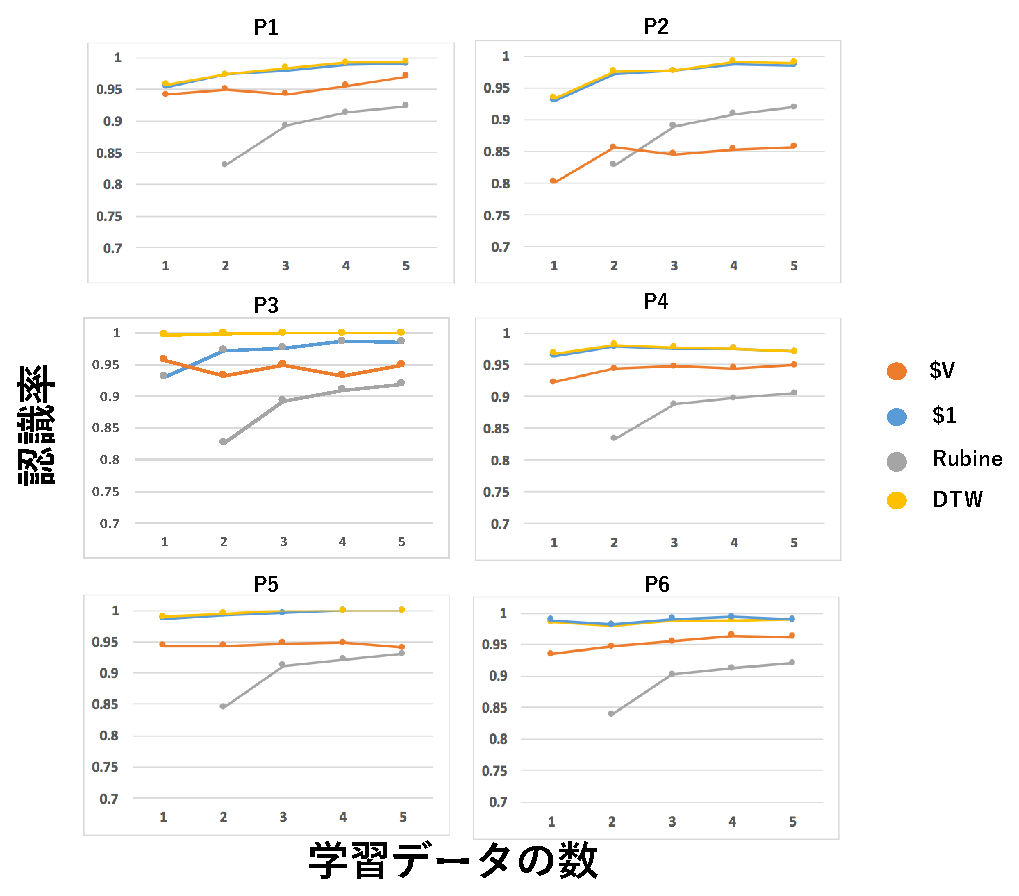
\includegraphics[width=1.0\columnwidth]{img/rec_rate.eps}
\caption{各手法における,被験者ごとの認識率の平均}
\label{fig:rec_rate}
\end{figure}

図\ref{fig:rec_rate}に各手法ごとの認識率の結果を示す.
それぞれの被験者の平均は,\$Vは93\%~(SD=4.55),\$1は98\%~(1.04),DTWは98\%~(0.86),Rubineは88\%~(2.14)であった.\$Vは\$1とDTWに対し,有意に低かった(p $<$ 0.01)が,被験者P1,P3,P4,P5,P6に関しては認識率の平均は95\%~(1.27)と高く,\$1と比べて認識率の低下を最小限に抑えることができた.\$Vは\$1とは異なり,大きさ,向き,位置に関して異なる手書きジェスチャを識別可能であるにもかかわらず,被験者P1,P3,P4,P5,P6に関しては,認識率はおよそ3\%しか低下しなかった.Rubineと比較した場合は,P1,P3,P4,P5,P6に関しては\$Vは有意に高かった(p $<$ 0.001).また,重み付けをしない場合と比べても,\$Vは全被験者について認識率は向上した.

P2の認識率が低かったのは,P2は別の名前のジェスチャで,形状が酷似したジェスチャが複数存在したため,識別が困難になったことが要因であると考えられる.また,\$Vは学習データに比例して認識率が高くなるとは言えない.これは,同じジェスチャの学習データを追加するたびに,大きさ,向き,位置それぞれの特徴量を算術平均するため,必ずしも入力データに類似する学習データが存在する可能性が高くなるとは言えないからである.しかしながら,ほとんどの被験者において,少ない学習データにおいて高い認識率を示し,学習データが1つの場合における,全ジェスチャセットの認識率の平均は91.2\%(SD=0.07),学習データが2つの場合は92.2\%(0.04),学習データが3つの場合は92.7\%(0.05),学習データが4つの場合は93.3\%(0.04),学習データが5つの場合は93.2\%(0.05)となった.

\newpage
\subsection{認識速度}
\begin{figure}[!h]
\centering
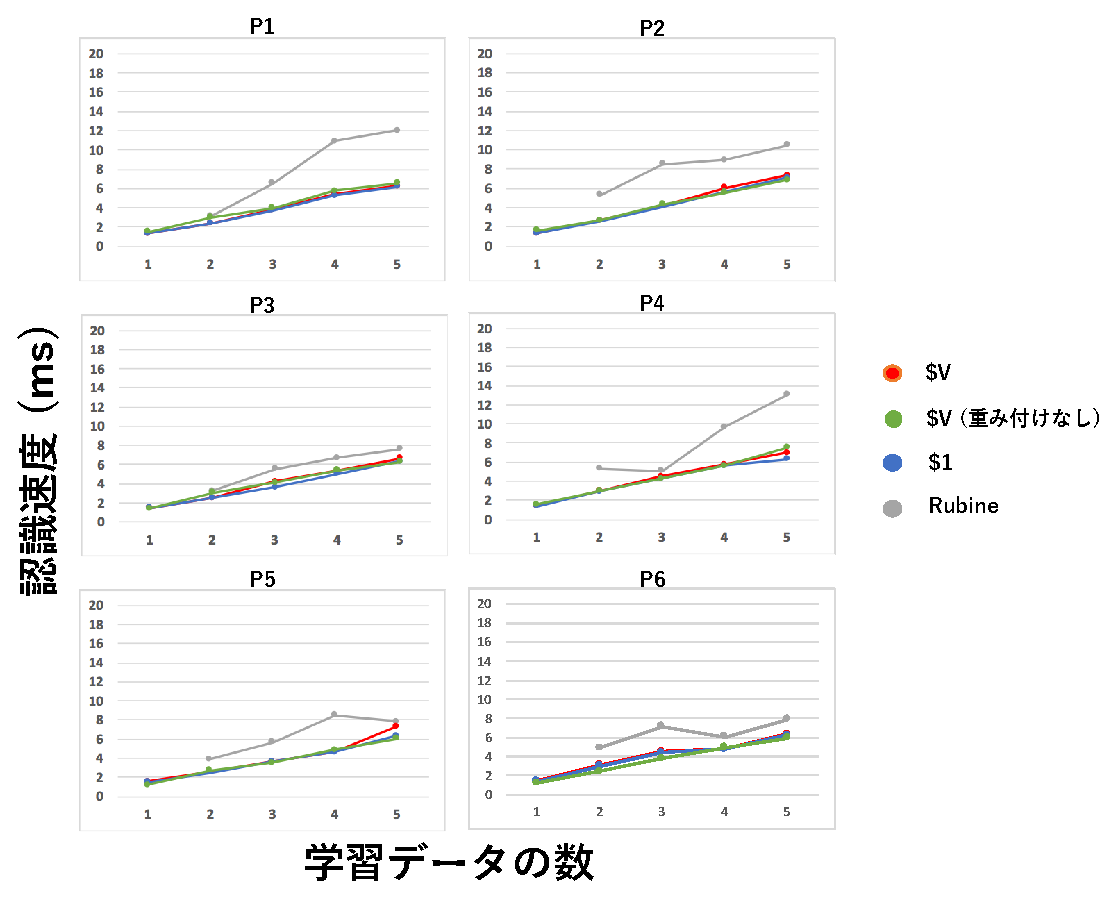
\includegraphics[width=1.0\columnwidth]{img/rec_speed.eps}
\caption{\$V,\$1,Rubineにおける,被験者ごとの認識速度の平均}
\label{fig:rec_speed}
\end{figure}

\begin{figure}[!h]
\centering
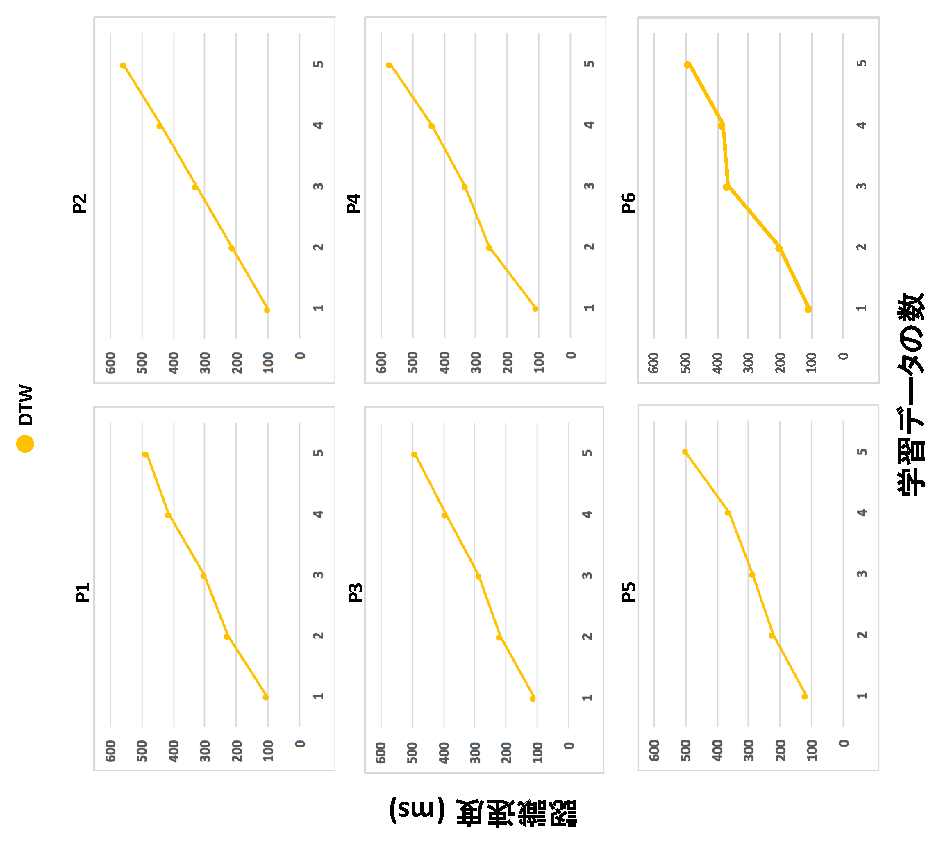
\includegraphics[width=1.0\columnwidth]{img/rec_speed_dtw.eps}
\caption{DTWにおける,被験者ごとの認識速度の平均}
\label{fig:rec_speed_dtw}
\end{figure}

図\ref{fig:rec_speed}に,\$V,\$1,Rubineの,図\ref{fig:rec_speed_dtw}に,DTWのジェスチャ1つを認識するまでの認識速度の結果を示す.
\$Vの認識速度は,全被験者の平均が,学習データの数が1つの場合~2.6ms (SD=0.2),学習データの数が2つの場合~3.5ms (0.3),学習データの数が3つの場合~4.1ms (0.3),学習データの数が4つの場合~4.9ms (0.3),学習データの数が5つの場合~6.1ms (0.4)となり非常に速いと言える.また,\$1と認識速度に有意差はなく~(p $<$ 0.001),\$Vは\$1と比べて認識速度の低下を抑えることに成功した.Rubineと比べると有意に速かった~(p $<$ 0.005).DTWの認識速度は図\ref{fig:rec_speed_dtw}に示すように非常に遅く,\$Vの認識速度はDTWのおよそ100分の1であった.
また,学習データに比例して認識速度が遅くなることも分かった.

\clearpage
\subsection{識別性能の結果}
\$Vの識別性能の結果を,N-best Listの1番目と2番目のスコアの差及びジェスチャが正しく認識された時の類似度及びジェスチャが正しく認識された時の類似度の最小値を示すことによって述べる.

図\ref{fig:rec_diff}に\$VにおけるN-best Listの1番目と2番目のスコアの差,図\ref{fig:rec_sim}に\$Vにおけるジェスチャが正しく認識された時の類似度,図\ref{fig:rec_min}に\$Vにおけるジェスチャが正しく認識された時の類似度の最小値の結果を示す.
N-best Listの1番目と2番目のスコアの差について,全ジェスチャセットの平均値はおよそ0.24~(SD = 0.10)となった.また,ジェスチャが正しく認識された時の類似度の平均値は0.94~(SD=0.04)となり非常に高いと言えるが,ジェスチャが正しく認識された時の類似度の最小値は被験者によってばらつきが生じ,平均値はおよそ0.83~(0.14)であった.また,N-best Listの1番目と2番目のスコアの差は,重み付けをしない場合と比べて有意に高く~(p $<$ 0.01),識別性能が向上したと言える.しかしながら,ジェスチャが正しく認識された時の類似度の最小値は,重み付けをしない場合と比べて有意に低かった~(p $<$ 0.01).これは,ジェスチャグループによっては,適した重み付けがされていない場合があり,その場合類似度が低くなるからであると考えられる.以上を踏まえ,%ジェスチャが正しく認識された時の類似度の平均値が高いことから,
重み付けは多くのジェスチャグループにおいて適用可能であるが,適用することによって類似度が低下する場合もあることがわかった.
また,ジェスチャが一致した時の類似度の最小値の平均は0.65以上であり,N-best Listの1番目と2番目のスコアの差の平均値は0.15以上であることから,認識のための類似度の閾値を0.5とすることによって,ジェスチャが一致するか否かを判別することが可能となると言える.
%\subsubsection{N-best Listsの1番目と2番目のスコアの差}
\begin{figure}[!h]
\centering
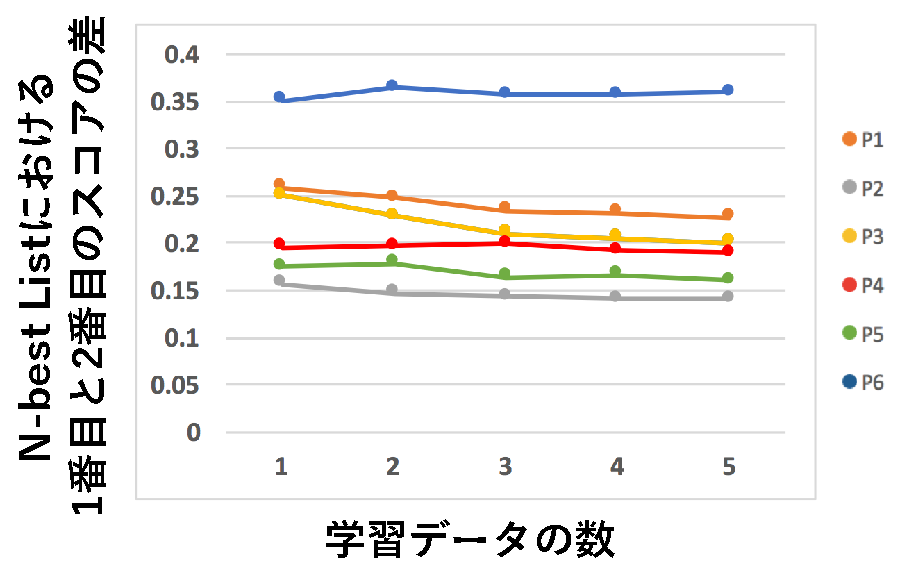
\includegraphics[width=0.7\columnwidth]{img/rec_diff.eps}
\caption{\$Vにおける,N-best Listの1番目と2番目のスコアの差の平均}
\label{fig:rec_diff}
\end{figure}

%\subsubsection{ジェスチャが正しく認識された時の類似度}
\begin{figure}[!h]
\centering
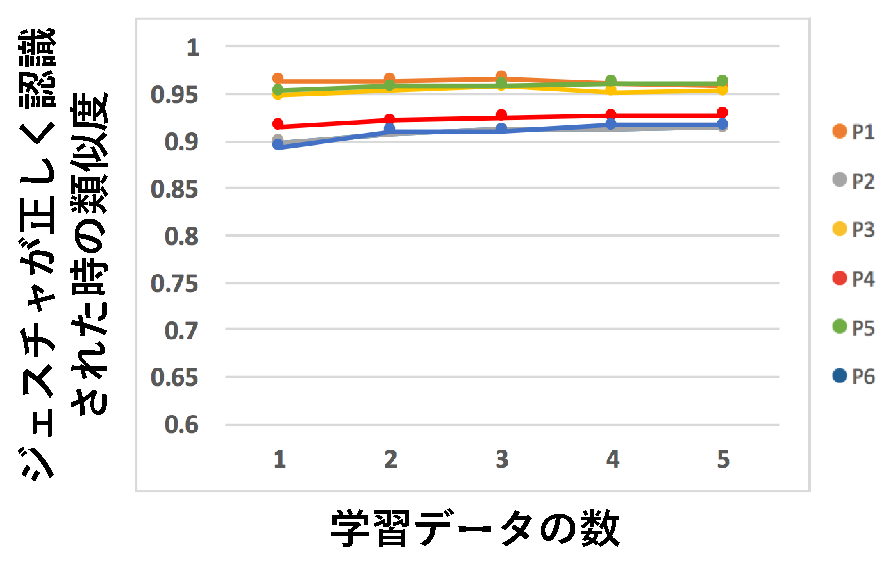
\includegraphics[width=0.7\columnwidth]{img/rec_sim.eps}
\caption{\$Vにおける,ジェスチャが正しく認識された時の類似度の平均}
\label{fig:rec_sim}
\end{figure}

%subsubsection{ジェスチャが正しく認識された時の類似度の最小値}
\begin{figure}[!h]
\centering
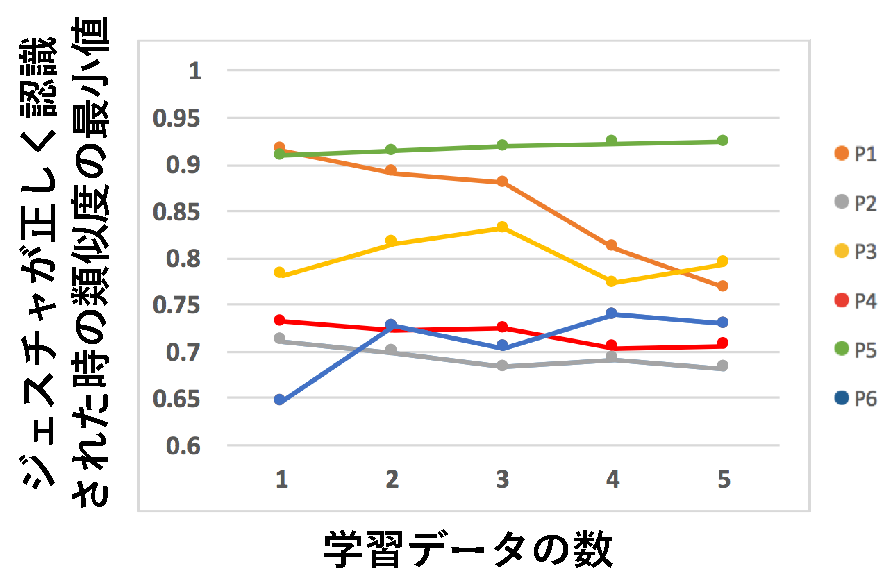
\includegraphics[width=0.7\columnwidth]{img/rec_min.eps}
\caption{\$Vにおける,ジェスチャが正しく認識された時の類似度の最小値の平均}
\label{fig:rec_min}
\end{figure}

\clearpage
以上を踏まえ,ジェスチャグループを作成し,ジェスチャグループ内に存在する学習データのみに対し,大きさ,向き,位置の類似度計算をすると認識速度の低下を防ぐことができるという仮説及び,同一ジェスチャグループ内において,他の学習データと類似している特徴量は,認識のための特徴量として用いなければ,認識率の低下を防ぐことができるという仮説は検証され,\$Vは,認識率及び認識速度において高いパフォーマンスを示し,かつ,形状や書き順が同じ手書きジェスチャを大きさ,向き,位置に関して識別可能なアルゴリズムであると言える.

%\TODO{学習データを追加する際の計算量を計測}
